\documentclass{beamer}[10]

\usepackage{graphicx}
\usepackage{xcolor}
\usepackage{tabto}
%\usepackage{beamerthemesplit}
\usepackage{tikz}
\usepackage{cancel}
\usepackage{verbatim}
\usepackage{fancybox}
\usepackage{enumerate}
\usepackage{amsmath,amssymb,amsthm,textcomp,mathtools}
\usepackage[super]{nth}
\usepackage[amssymb]{SIunits}
\usepackage{booktabs}
\usepackage{cancel}
\usepackage{bm}
\usepackage[utf8]{inputenc}
\usepackage{tabularx}
\usepackage{ragged2e}
\newcolumntype{Y}{ >{\RaggedRight\arraybackslash}X}
\usetikzlibrary{arrows,shapes}
\newcommand\T{\rule{0pt}{2.6ex}}
\newcommand\B{\rule[-1.2ex]{0pt}{0pt}}
\definecolor{UUcrimson}{RGB}{204,0,0}
\mode<presentation>
{ \usetheme{default}
  \usecolortheme[named=UUcrimson]{structure}
  \useinnertheme{circles}
  \setbeamercovered{transparent}
  \setbeamertemplate{blocks}[rounded]
  \usefonttheme[onlymath]{serif}
  \setbeamertemplate{navigation symbols}{}
  \setbeamertemplate{footline}[page number]
  \setbeamertemplate{navigation symbols}{}
  \setbeamercolor{section in toc}{fg=black,bg=white}
  \setbeamercolor{alerted text}{fg=UUcrimson!80!gray}
  \setbeamercolor*{palette primary}{fg=white,bg=UUcrimson}
  \setbeamercolor*{palette secondary}{fg=UUcrimson!70!black,bg=gray!15!white}
  \setbeamercolor*{palette tertiary}{bg=UUcrimson!80!black,fg=gray!10!white}
  \setbeamercolor*{palette quaternary}{fg=UUcrimson,bg=gray!5!white}
  \setbeamercolor*{palette sidebar primary}{fg=UUcrimson!10!black}
  \setbeamercolor*{palette sidebar secondary}{fg=white}
  \setbeamercolor*{palette sidebar tertiary}{fg=UUcrimson!50!black}
  \setbeamercolor*{palette sidebar quaternary}{fg=gray!10!white}
  \setbeamercolor{titlelike}{parent=palette primary,fg=white}
  \setbeamercolor{frametitle}{bg=UUcrimson}
  \setbeamercolor{frametitle right}{bg=UUcrimson}
  \setbeamercolor*{separation line}{}
  \setbeamercolor*{fine separation line}{}
}

\usetikzlibrary{backgrounds}
\makeatletter
\tikzstyle{every picture}+=[remember picture]
\tikzset{%
  fancy quotes/.style={
    text width=\fq@width pt,
    align=justify,
    inner sep=1em,
    anchor=north west,
    minimum width=\linewidth,
    font=\itshape
  },
  fancy quotes width/.initial={.8\linewidth},
  fancy quotes marks/.style={
    scale=8,
    text=white,
    inner sep=0pt,
  },
  fancy quotes opening/.style={
    fancy quotes marks,
  },
  fancy quotes closing/.style={
    fancy quotes marks,
  },
  fancy quotes background/.style={
    show background rectangle,
    inner frame xsep=0pt,
    background rectangle/.style={
      fill=gray!25,
      rounded corners,
    },
  }
}
\newenvironment{fancyquotes}[1][]{%
\noindent
\tikzpicture[fancy quotes background]
\node[fancy quotes opening,anchor=north west] (fq@ul) at (0,0) {``};
\tikz@scan@one@point\pgfutil@firstofone(fq@ul.east)
\pgfmathsetmacro{\fq@width}{\linewidth - 2*\pgf@x}
\node[fancy quotes,#1] (fq@txt) at (fq@ul.north west) \bgroup}
{\egroup;
\node[overlay,fancy quotes closing,anchor=east] at (fq@txt.south east) {''};
\endtikzpicture}
\makeatother


\usetikzlibrary{backgrounds}
\makeatletter
\tikzstyle{every picture}+=[remember picture]
\tikzset{%
  fancy defs/.style={
    text width=\fq@width pt,
    align=justify,
    inner sep=0.25em,
    anchor=north west,
    minimum width=\linewidth,
    font=\itshape
  },
  fancy defs width/.initial={.8\linewidth},
  fancy defs marks/.style={
    scale=8,
    text=white,
    inner sep=0pt,
  },
  fancy defs opening/.style={
    fancy defs marks,
  },
  fancy defs closing/.style={
    fancy defs marks,
  },
  fancy defs background/.style={
    show background rectangle,
    inner frame xsep=0pt,
    background rectangle/.style={
      fill=gray!25,
      rounded corners,
    },
  }
}
\newenvironment{fancydefs}[1][]{%
\noindent
\tikzpicture[fancy defs background]
\node[fancy defs opening,anchor=north west] (fq@ul) at (0,0) {};
\tikz@scan@one@point\pgfutil@firstofone(fq@ul.east)
\pgfmathsetmacro{\fq@width}{\linewidth - 2*\pgf@x}
\node[fancy defs,#1] (fq@txt) at (fq@ul.north west) \bgroup}
{\egroup;
\node[overlay,fancy defs closing,anchor=east] at (fq@txt.south east) {};
\endtikzpicture}
\makeatother
\usepackage{scalerel}[2014/03/10]
\usepackage{stackengine}
\usepackage{empheq}
\newcommand*\widefbox[1]{\fbox{\hspace{0.5em}#1\hspace{0.5em}}}

\newcommand\reallywidetilde[1]{\ThisStyle{%
  \setbox0=\hbox{$\SavedStyle#1$}%
  \stackengine{-.1\LMpt}{$\SavedStyle#1$}{%
    \stretchto{\scaleto{\SavedStyle\mkern.2mu\sim}{.5467\wd0}}{.4\ht0}%
%    .2mu is the kern imbalance when clipping white space
%    .5467++++ is \ht/[kerned \wd] aspect ratio for \sim glyph
  }{O}{c}{F}{T}{S}%
}}
\usepackage{media9}

\logo{
\includegraphics[width=0.75cm]{logo.jpg}}
\author[Gibbs]{Dr. Jeremy A. Gibbs}
\institute{Department of Mechanical Engineering\\University of Utah}
\date{Spring 2017}
\title{Environmental Fluid Dynamics: Lecture 1}
% colors
\definecolor{colororange}{HTML}{E65100} % orange
\definecolor{colordgray}{HTML}{795548} % dark gray for note
\definecolor{colorhgray}{HTML}{212121} % heavy dark gray for normal text
\definecolor{colorgreen}{HTML}{009688} % green
\definecolor{colorwhite}{HTML}{FFFFFF} % background white
\definecolor{colorlgray}{HTML}{F5F3EE} % background light gray
\definecolor{colorblue}{HTML}{0277BB} % blue
\definecolor{colorred}{HTML}{CC0000} % red
\newcommand{\fontsizeone}{1.9em}

\newcommand{\framecard}[2][colorgreen]{
  {\setbeamercolor{background canvas}{bg=#1}
    \begin{frame}[plain]
    \vfill
    \begin{center}
     {#2}
    \end{center}
    \vfill
    \end{frame}
  }
}

\begin{document}

%----------------------------------------------------------------------------------------
%	TITLE & TOC SLIDES
%----------------------------------------------------------------------------------------

\begin{frame} 
  \titlepage
\end{frame}

%------------------------------------------------

\begin{frame}
\frametitle{Overview}
\tableofcontents
\end{frame}

%------------------------------------------------
\section{Syllabus} %
%------------------------------------------------
\framecard[colorred]{{\color{white}\Huge Syllabus}}

\subsection{Administrative}
\begin{frame}{Instructor}
How to contact me:

\begin{itemize}
\item Email: \href{mailto:jeremy.gibbs@utah.edu}{\color{UUcrimson}\underline{jeremy.gibbs@utah.edu}}
\item Office: MEK 2566
\item Hours: By appointment (email or stop by)
\end{itemize}
~\\~\\
Course websites:

\begin{itemize}
\item Canvas
\item \href{http://gibbs.science/efd}{\color{UUcrimson}\underline{http://gibbs.science/efd}}
\end{itemize}


\end{frame}

%------------------------------------------------

\begin{frame}{Meeting Times}
Class schedule:

\begin{itemize}
\item Class will be held in MEB 1225
\item Tues and Thurs, 10:45a - 12:05p
\item We will miss three classes:
\begin{itemize}
\item Thursday, Mar. 9 (travel)
\item Tuesday, Mar. 14 (spring break)
\item Tuesday, Mar. 16 (spring break)
\end{itemize}
\end{itemize}
\end{frame}

%------------------------------------------------

\begin{frame}{Textbooks}

Class lectures will primarily follow two textbooks:
\begin{itemize}
\item \textbf{\emph{An Introduction to Boundary Layer Meteorology}}\newline R.B. Stull (Kluwer, 1988), 670pp.
\item \textbf{\emph{Introduction to Micrometeorology, \nth{2} edition}}\newline S.P. Arya (Academic Press, 2001), 420 pp.
\end{itemize}
\end{frame}

%------------------------------------------------

\begin{frame}{Recommended Textbooks}

Other useful textbooks:
\begin{itemize}
\item \textbf{\emph{The Atmospheric Boundary Layer}}\newline J. R. Garratt (Cambridge University Press, 1992), 316 pp.
\item \textbf{\emph{Atmospheric Boundary Layer Flows}}\newline J.C. Kaimal and J.J. Finnigan (Oxford, 1994), 289 pp.
\item \textbf{\emph{Turbulence in the Atmosphere}}\newline J.C. Wyngaard (Cambridge University Press, 2010), 393 pp.
\item \textbf{\emph{Boundary Layer Climates, \nth{2} edition}}\newline T.R. Oke (Routledge, 1987), 435 pp.
\item \textbf{\emph{Handbook of Micrometeorology}}\newline X. Lee, W. Massman, and B. Law (Kluwer, 2004), 250 pp.
\end{itemize}
\end{frame}

%------------------------------------------------

\begin{frame}{Grading}
\begin{itemize}
\item Homework - 20\%
\item Midterm Exam - 25\%
\item Project \#1 - 20\%
\item Final Project - 35\%
\end{itemize}
\end{frame}

%------------------------------------------------
\subsection{Course Overview}
\begin{frame}{Course Description}
\begin{itemize}
\item An introduction to Environmental Fluid Dynamics focusing primarily on micrometeorological processes occurring in the atmospheric boundary layer (ABL; the lower 1-3 km of the troposphere)
\item Since this is the part of the atmosphere that humans are directly in contact with, it is of great importance to both engineers and atmospheric scientists.
\item For example, the small-scale motions responsible for pollution dispersion are related to surface fluxes of heat and momentum.
\end{itemize}

\end{frame}

%------------------------------------------------

\begin{frame}{Course Outline}
\textbf{Introduction}

\begin{itemize}
\item The ABL
	\begin{itemize}
		\item basic definitions and concepts
		\item scales of motion, diurnal cycles
		\item introduction to rotation and stratification
	\end{itemize}
	\item Equilibrium and departures from it
	\item Atmospheric thermodynamics
		\begin{itemize}
			\item potential temperature
			\item virtual potential temperature
			\item buoyancy frequency
			\item potential energy
		\end{itemize}
\end{itemize}
\end{frame}

%------------------------------------------------

\begin{frame}{Course Outline}
\textbf{Energy Balances}
\begin{itemize}
\item radiation characteristics
\item near-surface exchanges (fluxes)
\item near-surface energy budget
\end{itemize}
~\\
\textbf{Basic Equations}
\begin{itemize}
\item rotation, stratification, boundary layer simplifications
\end{itemize}
~\\
\textbf{Atmospheric Surface Layer Scaling}
\begin{itemize}
\item Monin-Obukhov similarity theory
\item Neutral, convective, and stable boundary layers
\end{itemize}
\end{frame}

%------------------------------------------------

\begin{frame}{Course Outline}
\textbf{Atmospheric Boundary Layer Turbulence}
\begin{itemize}
\item Intro to turbulence in the environment
	\begin{itemize}
		\item the critical effects of buoyancy on turbulence
		\item turbulent entrainment
		\item stability effects
	\end{itemize}
\item Measuring techniques
	\begin{itemize}
		\item intro to various measuring techniques including sonic anemometry, balloon borne measurements, and remote sensing techniques
	\end{itemize}
\item Analysis of turbulence data sets and application to a real world field experiment
\end{itemize}

\end{frame}

%------------------------------------------------

\begin{frame}{Course Outline}
\textbf{Inhomogeneous Boundary Layers}
\begin{itemize}
\item Vegetative canopies, urban fluid mechanics
\item Surface inhomogeneities
	\begin{itemize}
		\item roughness effects
		\item complex terrain
		\item urban
	\end{itemize}
\item Terrain-induced flows
\item Atmospheric dispersion concepts and models
\begin{itemize}
	\item simple Gaussian plume to Lagrangian dispersion models
\end{itemize}
\item Urban Heat Island
\end{itemize}

\end{frame}

%------------------------------------------------

\begin{frame}{Coursework - Homework and Exams}
\textbf{Homework}
\begin{itemize}
	\item Periodic homework assignments will be given during class and then posted on the web site and Canvas.  
	\item Homework will be collected in class and via Canvas on the due date. Late homework will generally not be accepted.
\end{itemize}

\textbf{Homework}
\begin{itemize}
	\item There will be one midterm exam
	\item The exam will consist of an in-class part and a take-home part.
\end{itemize}
\end{frame}

%------------------------------------------------

\begin{frame}{Coursework - Projects}
\textbf{Project \#1}
\begin{itemize}
	\item Goal is to obtain a working understanding of the Surface Energy Balance (SEB) for urban areas. 
	\item ou will model the urban SEB for a tower located in Murray, UT using the LUMPS (Local-scale Urban Meteorological Parameterization Scheme) model. 
	\item At the end of the project you will have a working simulation tool.
\end{itemize}

\textbf{Final Project}
\begin{itemize}
	\item You will investigate various aspects of turbulence by using data from recent field experiments.
	\item The project will consist of two parts: a written report and an oral presentation. You may work in groups of 2 or 3.
\end{itemize}
\end{frame}

%------------------------------------------------

\begin{frame}{Computing Skills}
All students are expected to have basic computing skills and knowledge of a programming language (FORTRAN, C, C++, Python, etc) or scientific computing software package (Maple, Matlab, EES, etc)
\end{frame}

%------------------------------------------------
\section{Introduction to EFD} %
%------------------------------------------------
\framecard[colorred]{{\color{white}\Huge Introduction to EFD}}
\subsection{Definitions and Applications}
%------------------------------------------------
\subsection*{Definitions}

\begin{frame}{Definitions}

{\large \textbf{Environmental Fluid Mechanics}}
\\\vspace{2pt}
\begin{fancydefs}
	principles that govern \textbf{transport}, \textbf{mixing}, and
	\textbf{transformation processes} in environmental fluids 
	(\textit{e.g.}, physical, biological, chemical)
	\\\\includes stratification and rotation
\end{fancydefs}
\end{frame}

%------------------------------------------------
\begin{frame}{Definitions}

{\large \textbf{Micrometeorology}}
\\\vspace{2pt}
\begin{fancydefs}
	atmospheric phenomena and processes at the smaller end of the spectrum of atmospheric scales and near the earth’s surface (atmospheric boundary layer - ABL)
	\\\\Fine scale structure is important
\end{fancydefs}
~\\~\\
{\large \textbf{Microclimatology}}
\\\vspace{2pt}
\begin{fancydefs}
	same physical scales much longer time averaging scales
\end{fancydefs}

\end{frame}

%------------------------------------------------

\begin{frame}{Definitions}

{\large \textbf{Environmental Fluid Dynamics}}
\\\vspace{2pt}
\begin{fancydefs}
	Integrates different aspects of Thermal-Fluids Science (not just fluid mechanics!)\\
	\begin{itemize}
		\item fluid mechanics
		\item thermodynamics
		\item heat transfer (conduction, convection, radiation)
		\item mass transfer
	\end{itemize}

\end{fancydefs}
\end{frame}

%------------------------------------------------
\begin{frame}{Applications}

\begin{itemize}
	\item Urban planning
	\begin{itemize}
		\item Air quality (pollutants, greenhouse gases, accidental releases)
		\item Water and energy budgets (``green'' infrastructure)
	\end{itemize}
	\item Defense strategies
	\begin{itemize}
		\item Toxic releases: biological, chemical, radiation
	\end{itemize}
	\item Agriculture and forest meteorology (evapotranspiration, water budget)
	\item Aeronautical meteorology
	\item Wind engineering
	\item Numerical weather prediction and climate simulations
	\item More ...
\end{itemize}

\end{frame}

%------------------------------------------------
\begin{frame}{Scales of Motion}

\begin{itemize}
	\item Synoptic scales (100+ $\kilo\metre$)
	\item Mesoscale (10-1000 $\kilo\metre$)
	\item Microscale ($<1$ $\metre$ - 10 $\kilo\metre$)
	\item Engineering scale (viscous - 10 $\metre$)
	\item Urban scale (1 $\metre$ - 100 $\kilo\metre$)
\end{itemize}

\begin{figure}
	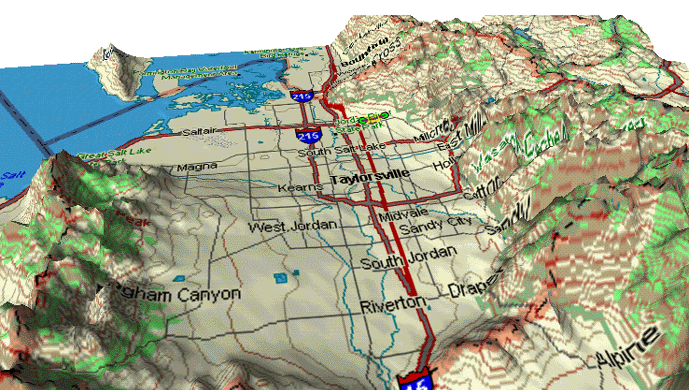
\includegraphics[width=0.8\textwidth]{scales1.png}
\end{figure}

\end{frame}

%------------------------------------------------
\begin{frame}{Time and Space Scales}

\begin{figure}
	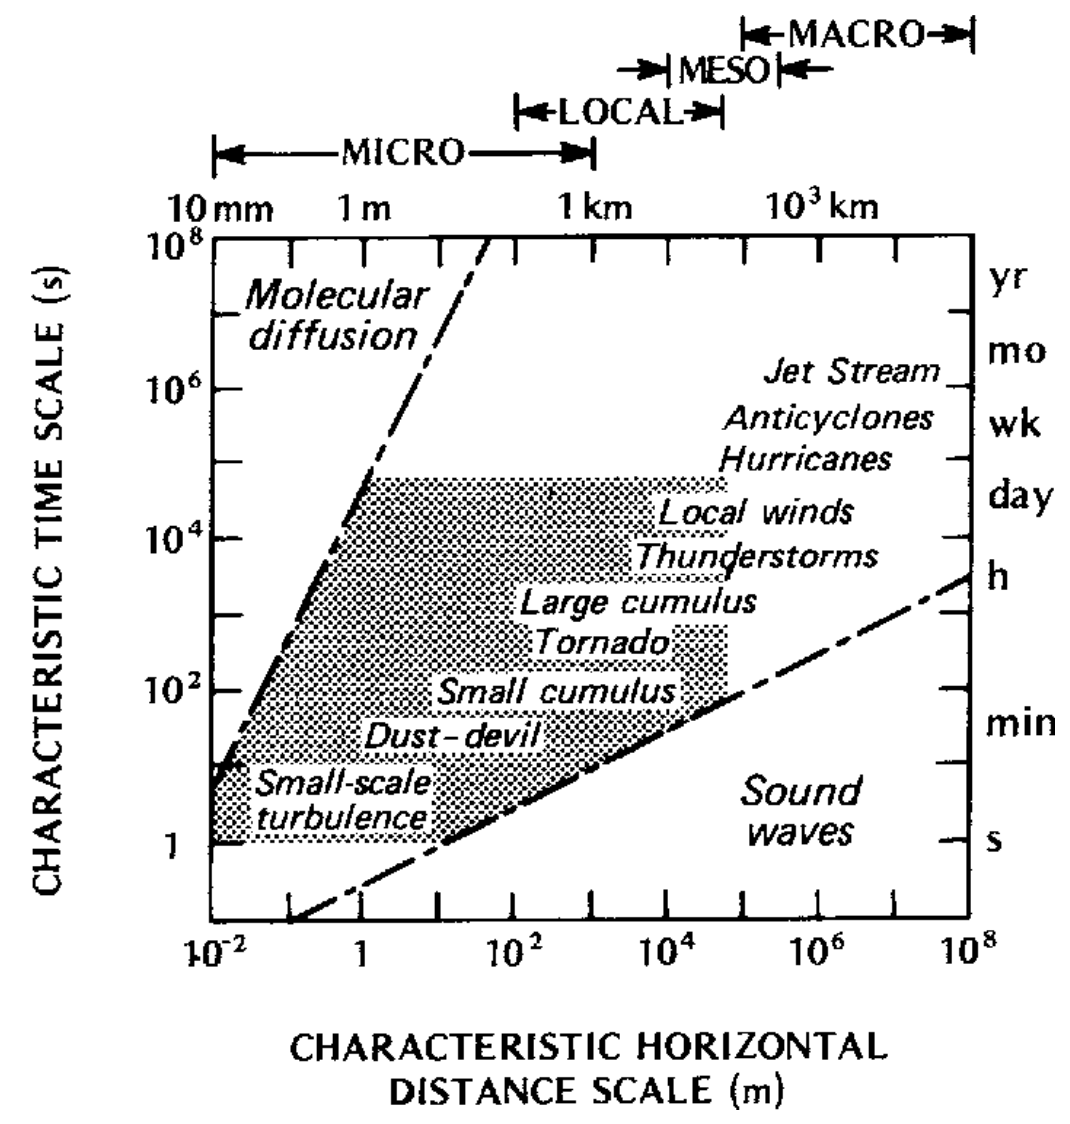
\includegraphics[width=0.65\textwidth]{scales2.png}
\end{figure}
\centering {\small from Boundary Layer Climates (Oke, 1987)}
\end{frame}

%------------------------------------------------
\begin{frame}{Time and Space Scales}

\begin{figure}
	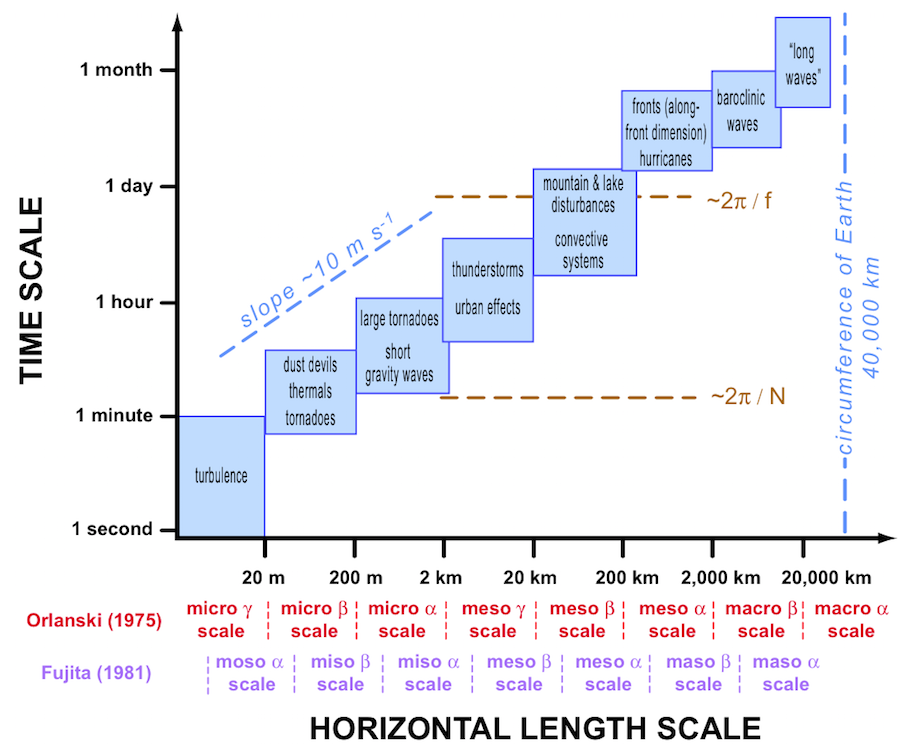
\includegraphics[width=0.8\textwidth]{scales3.png}
\end{figure}
\centering {\small from Mesoscale Meteorology (Markowski and Richardson, 2010)}
\end{frame}

%------------------------------------------------
\begin{frame}{Time and Space Scales}

\begin{figure}
	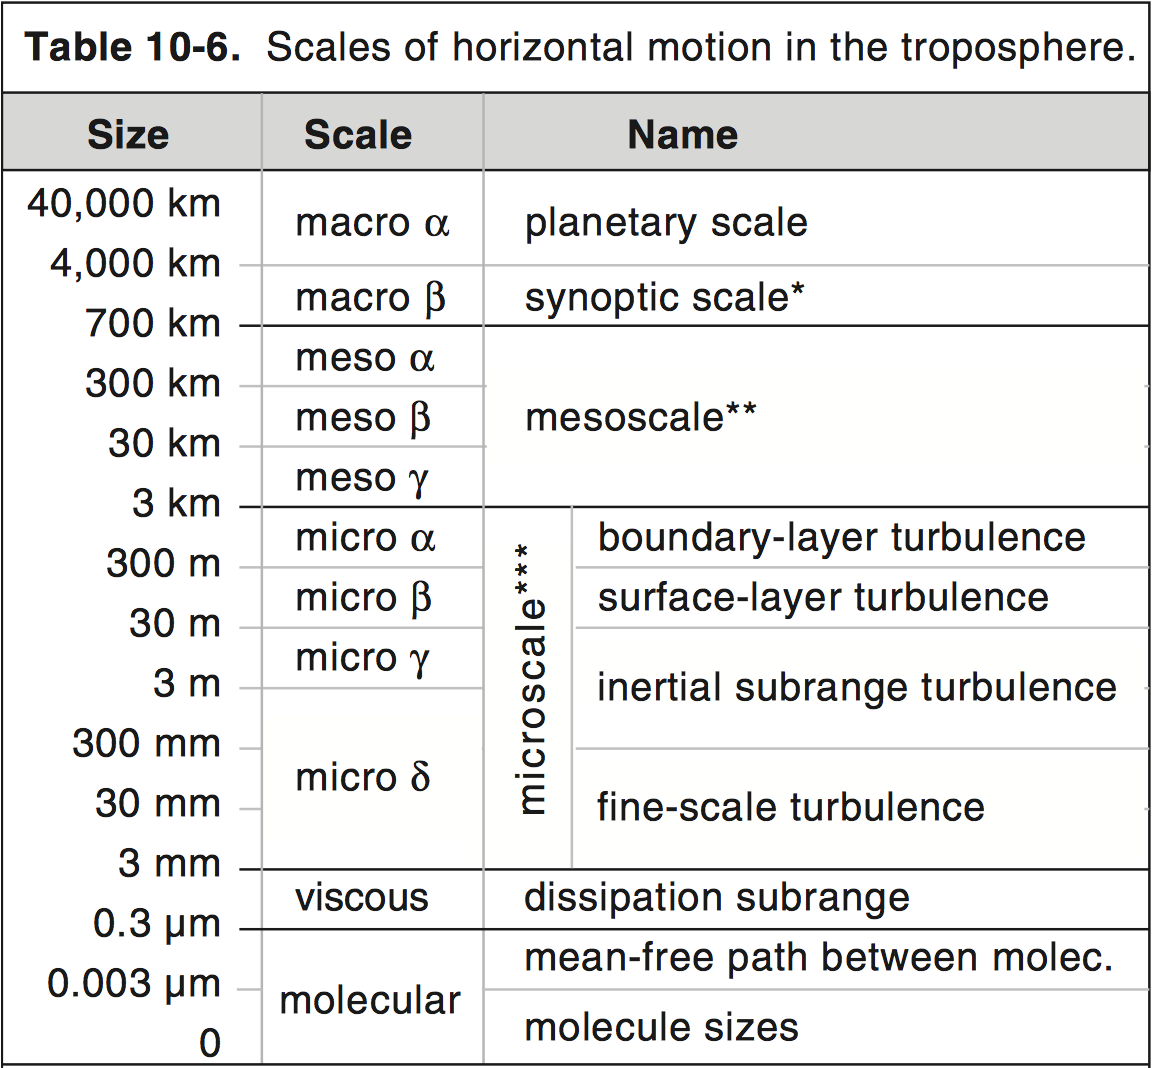
\includegraphics[width=0.725\textwidth]{scales4.png}
\end{figure}
\centering {\small from Meteorology for Engineers and Scientists (Stull)}
\end{frame}

%------------------------------------------------
\subsection{Atmospheric Boundary Layer}
\begin{frame}{Boundary Layer Research}
\textbf{Aerodynamic Boundary Layer}
\begin{itemize}
	\item 1870s – Froude carried out tow tank experiments to study friction over a flat plate
	\item 1905 – ``boundary layer'' - likely coined by Prandtl - thin region of the flow near the wall where frictional effects are confined
	\item 1908 Blasius solution – laminar boundary layer
\end{itemize}
\end{frame}

%------------------------------------------------
\begin{frame}{Boundary Layer Research}

{\large \textbf{Atmospheric Boundary Layer}}
\begin{fancydefs}
	the part of troposphere that is directly influenced
	by the presence of the earth surface and responds
	to surface forcings with a timescale of about an
	hour or less
\end{fancydefs}

Characterized by well developed mixing (turbulence) generated by
\begin{itemize}
	\item the atmosphere moving across Earth’s rough surface (\textit{mechanically driven turbulence})
	\item by the bubbling up of air parcels from the heated earth (\textit{buoyancy driven turbulence})
\end{itemize}
~\\
This turbulence is responsible for much of the heat transfer from the earth's surface to the atmosphere (\textit{sensible heat flux})
\end{frame}

%------------------------------------------------
\begin{frame}{Atmospheric Boundary Layer}

\begin{figure}
	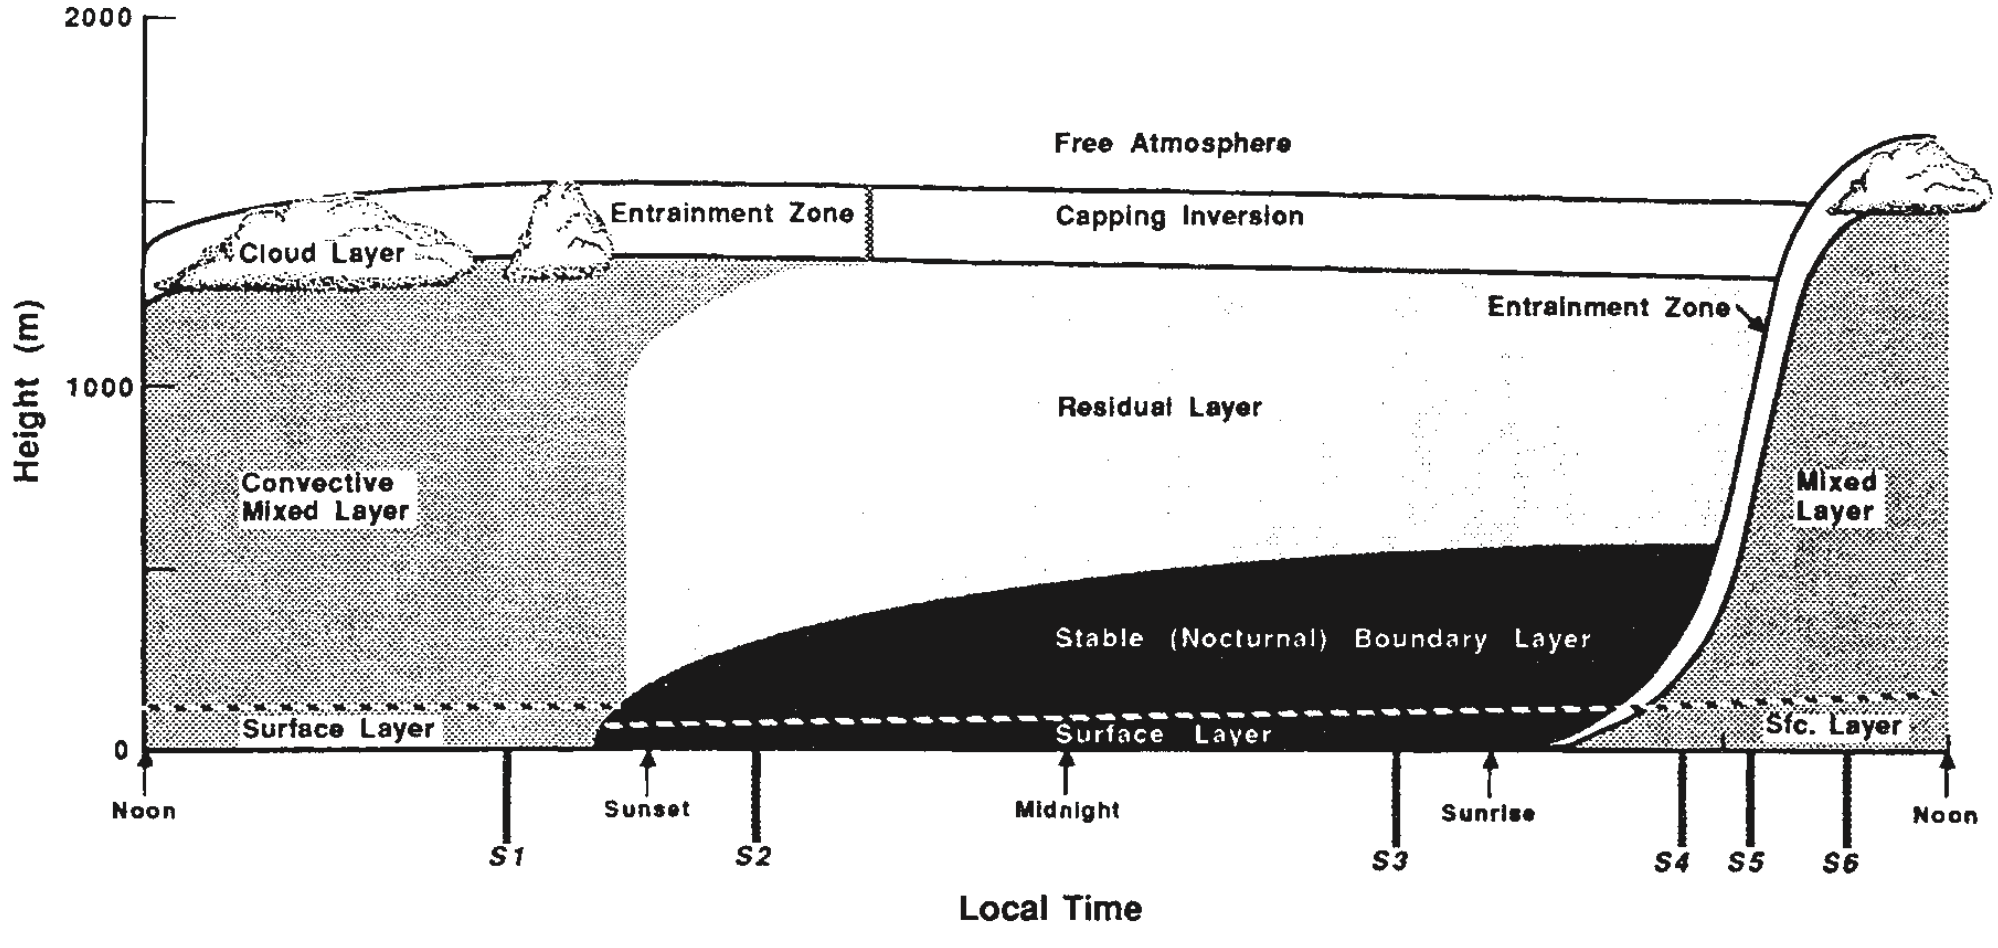
\includegraphics[width=1\textwidth]{abl1.png}
\end{figure}
\centering {\small Diurnal cycle of ABL over simple terrain (from Stull 1988)}
\end{frame}

%------------------------------------------------
\begin{frame}{Atmospheric Boundary Layer}

Daytime convective boundary layer (CBL) sub-layers
\begin{figure}
	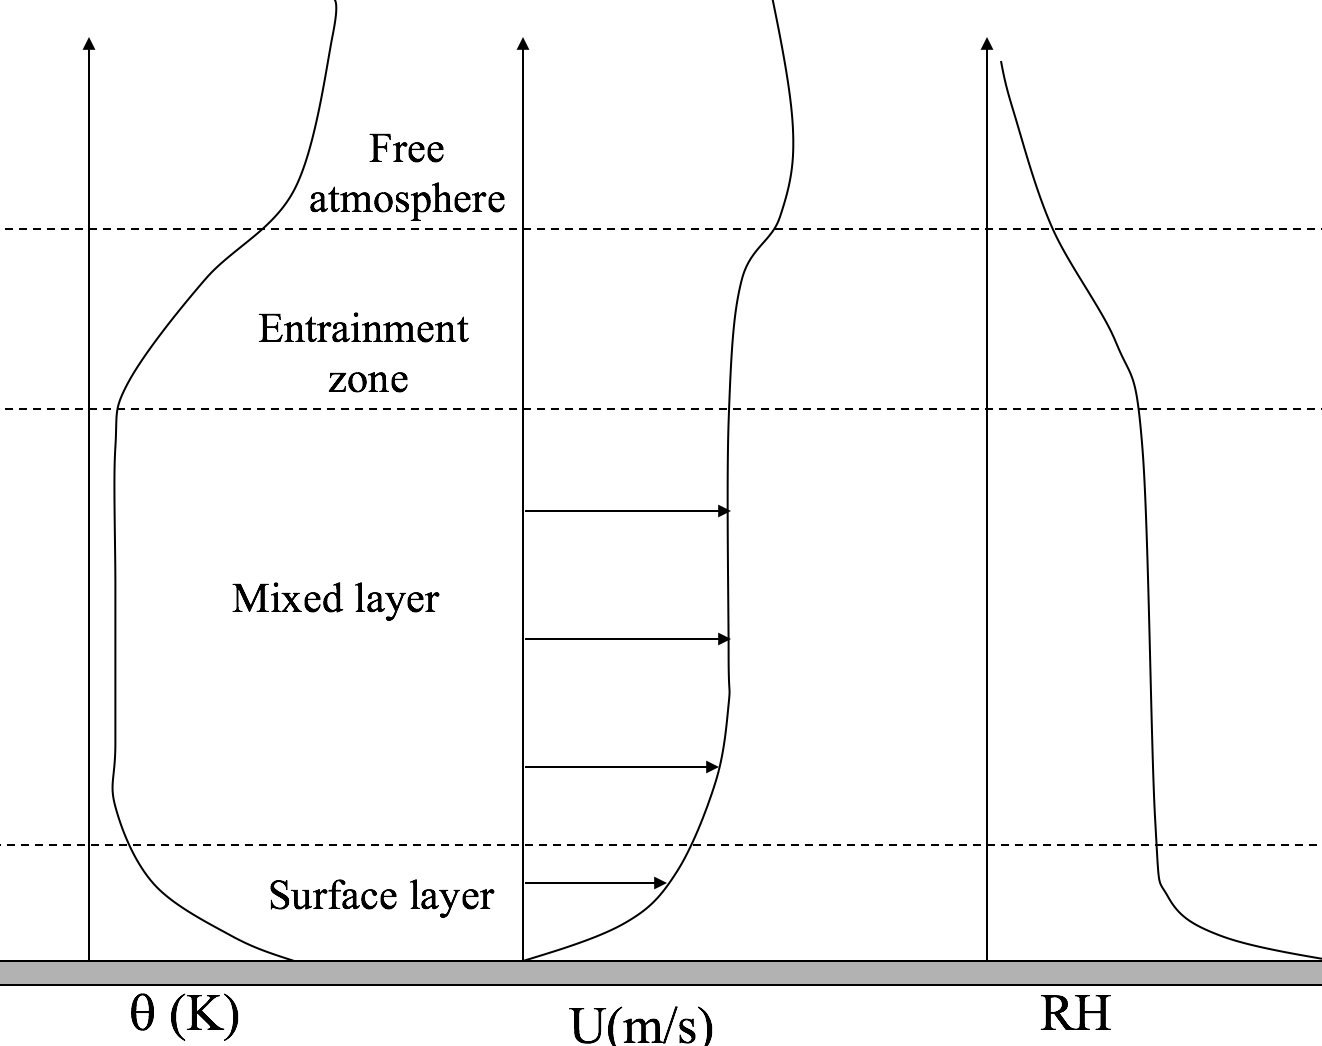
\includegraphics[width=0.9\textwidth]{abl2.png}
\end{figure}
\end{frame}

%------------------------------------------------
\begin{frame}{Atmospheric Boundary Layer}

\begin{figure}
	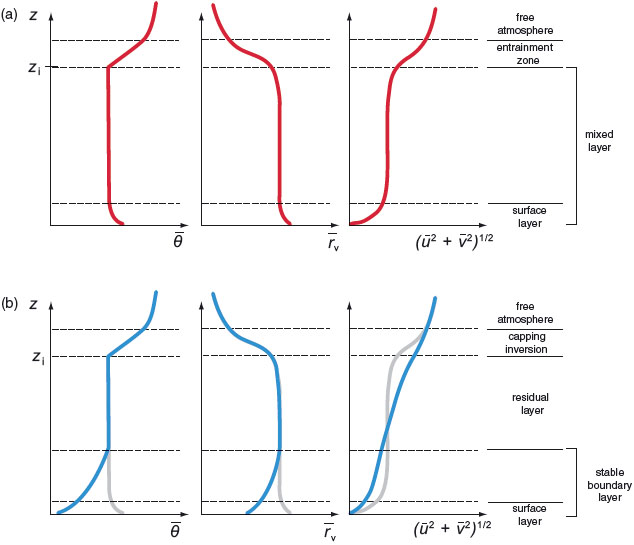
\includegraphics[width=0.8\textwidth]{abl3.jpg}
\end{figure}
\centering {\small from Markowski and Richardson (2010)}
\end{frame}

%------------------------------------------------
\begin{frame}{Atmospheric Boundary Layer}
\begin{figure}
	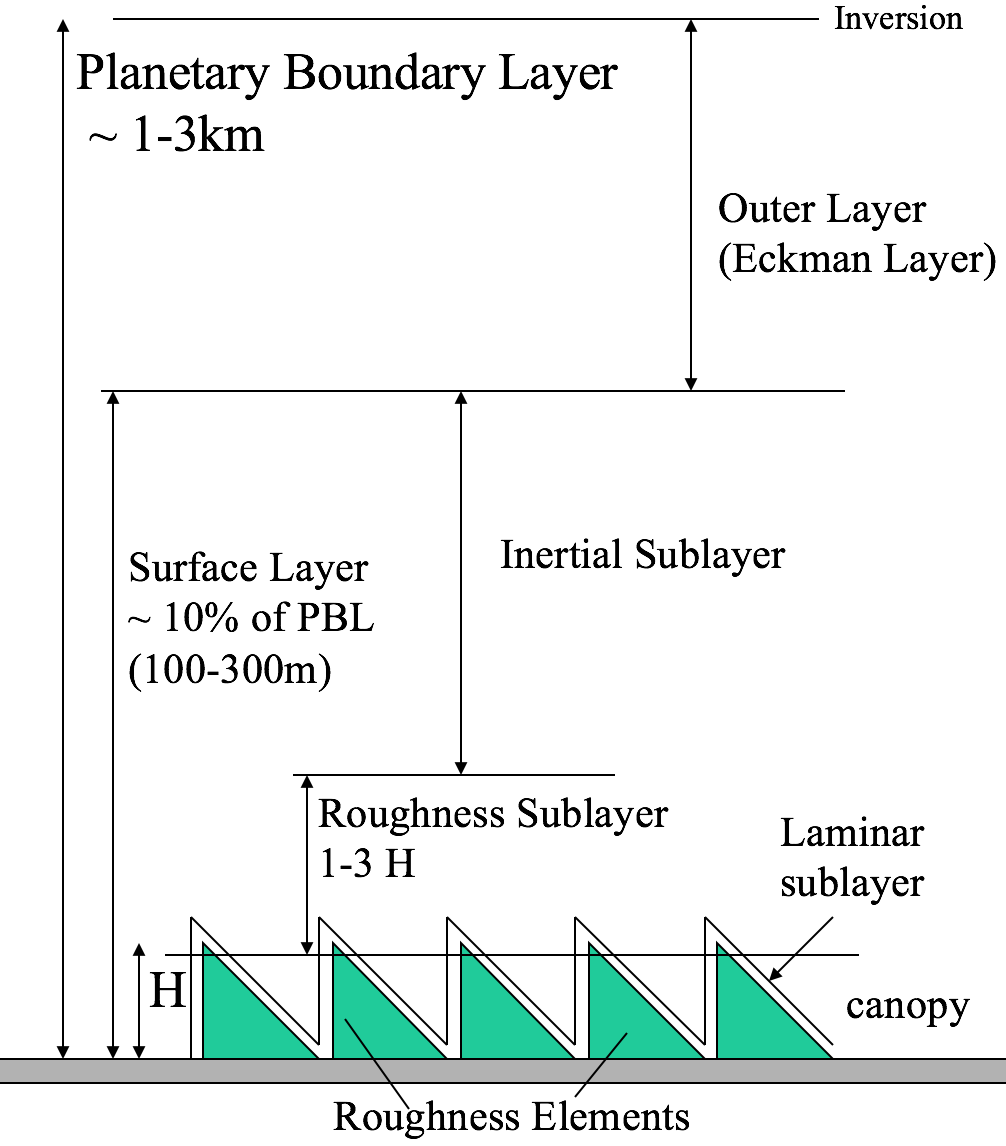
\includegraphics[width=0.65\textwidth]{abl4.png}
\end{figure}
\end{frame}

%------------------------------------------------
\begin{frame}{Atmospheric Surface Layer}

\textbf{Inertial sub-layer }
\begin{itemize}
	\item variation in vertical fluxes $<10$\%
	\item log-law wind profile
\end{itemize}

\textbf{Roughness sub-layer }
\begin{itemize}
	\item $\mathcal{O}(H)$
	\item horizontal heterogeneity
\end{itemize}

\textbf{Laminar sub-layer }
\begin{itemize}
	\item $< 1-2$ mm
\end{itemize}
\end{frame}

%------------------------------------------------
\begin{frame}{Our scales of interest}
In this Environmental Fluid Dynamics class, we will focus on the following scales:
\begin{itemize}
	\item Vertical: $< 3\ \kilo\metre$
	\item Horizontal $< 50\ \kilo\metre$ (micro- to mesoscale)
	\item Time scale $\sim 1$ day
\end{itemize}

We will also examine night vs. day

\end{frame}

%------------------------------------------------
\begin{frame}{ABL Transport}
\textbf{Mass}
\begin{itemize}
	\item pollutants – particles
	\item water
	\item biological process - pollen
\end{itemize}

\textbf{Heat}
\begin{itemize}
	\item sensible heat flux
	\item latent heat flux
\end{itemize}

\textbf{Momentum}
\begin{itemize}
	\item Surface drag - urban vs. rural vs. body of water
\end{itemize}
Each of these also has spatial variability
~\\~\\
We will need to develop equations to describe these processes!
\end{frame}

%------------------------------------------------
\begin{frame}{Stratification}

\begin{itemize}
	\item Variation of density with space
	\item Most introductory Engineering Fluid Mechanics classes focus on constant density problem or ``neutral'' boundary layers
	\item We will mostly consider $\rho = \rho(z)$
	\item The density variation in the atmosphere will typically be dominated by variations in temperature and humidity
\end{itemize}

\end{frame}

%------------------------------------------------
\begin{frame}{Rotation}
For much of the class we will neglect rotation effects, but when is rotation important?
~\\~\\
Let's introduce the \textbf{Rossby Number}
$$
\mathrm{Ro} = \frac{\text{inertial}}{\text{rotational}} = \frac{U}{fL_R}
$$
where
\begin{align*}
	f& = 2\Omega \sin\phi\qquad &\text{Coriolis parameter}&\\
	\phi &= \text{latitude}\\
	\Omega &= 7.292 \times 10^5 \radian\reciprocal\second \qquad &\text{Angular speed of Earth}&\\
	L_R &= \text{relevant length scale}
\end{align*}
If $\mathrm{Ro} \gg 1$, rotation is assumed negligible (\textit{i.e.} Coriolis acceleration is less than ``horizontal'' acceleration)
\end{frame}

%------------------------------------------------
\begin{frame}{Field Experiments}
\begin{figure}
	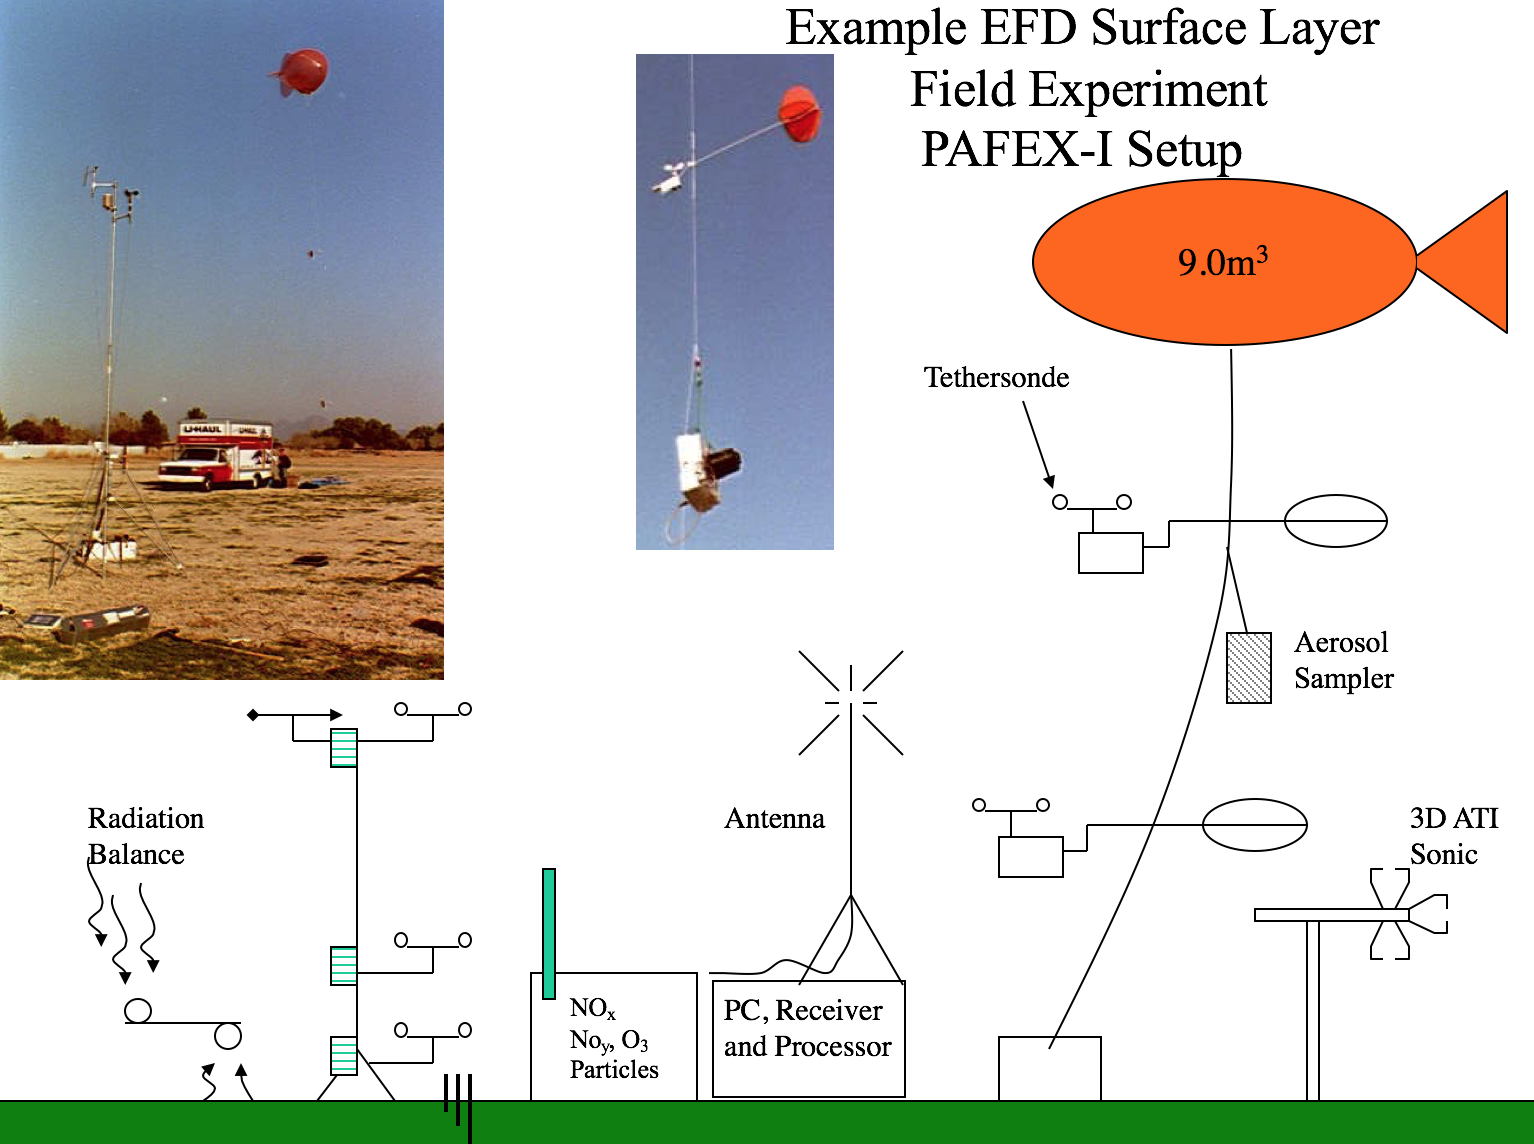
\includegraphics[width=1\textwidth]{materhorn1.png}
\end{figure}
\end{frame}

%------------------------------------------------
\begin{frame}{Field Experiments: MATERHORN}
172 Towers + 90 Sonic Anemometers
\begin{figure}
	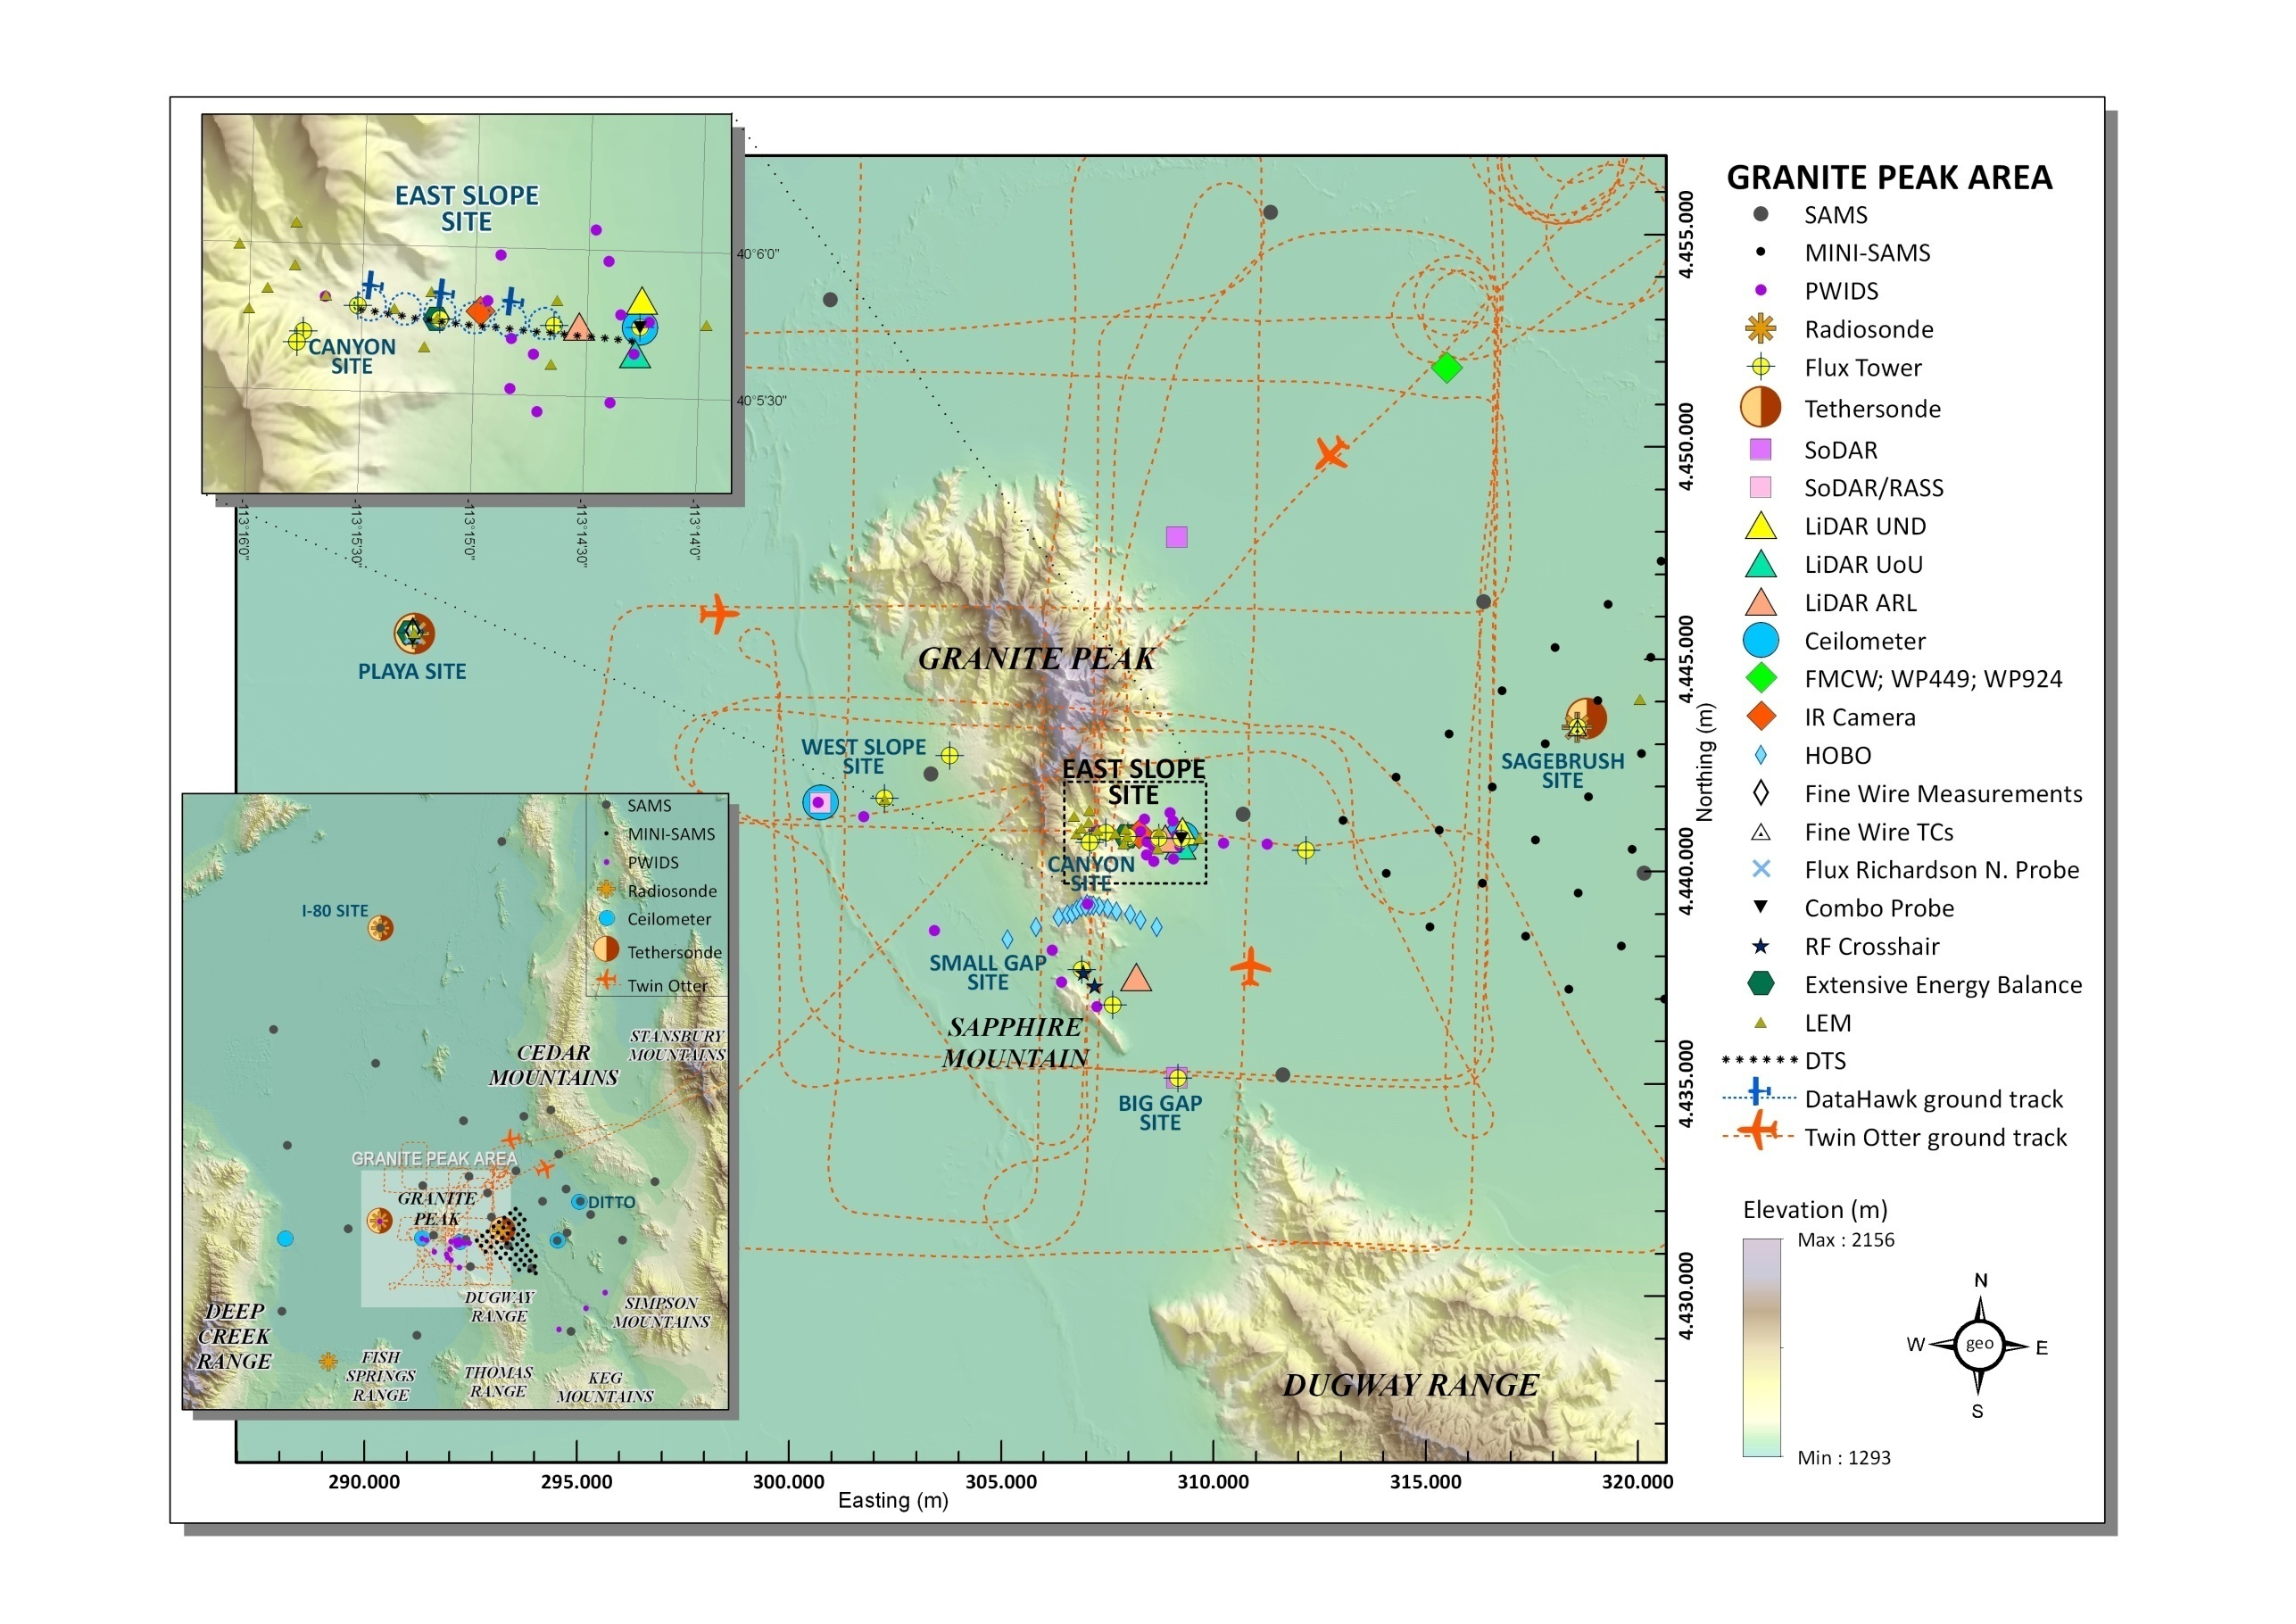
\includegraphics[width=1\textwidth]{materhorn2.png}
\end{figure}
\end{frame}

%------------------------------------------------
\subsection{Surface Energy Balance}
\begin{frame}{Basic Surface Energy Balance Ideas}
We will expand on these ideas later as we derive formal transport equations for responsive fluxes
~\\~\\
These initial ideas will allow us to understand the basic mechanisms of heat transfer near the surface of the earth
\end{frame}

%------------------------------------------------
\begin{frame}{Basic Surface Energy Balance Ideas}
\begin{figure}
	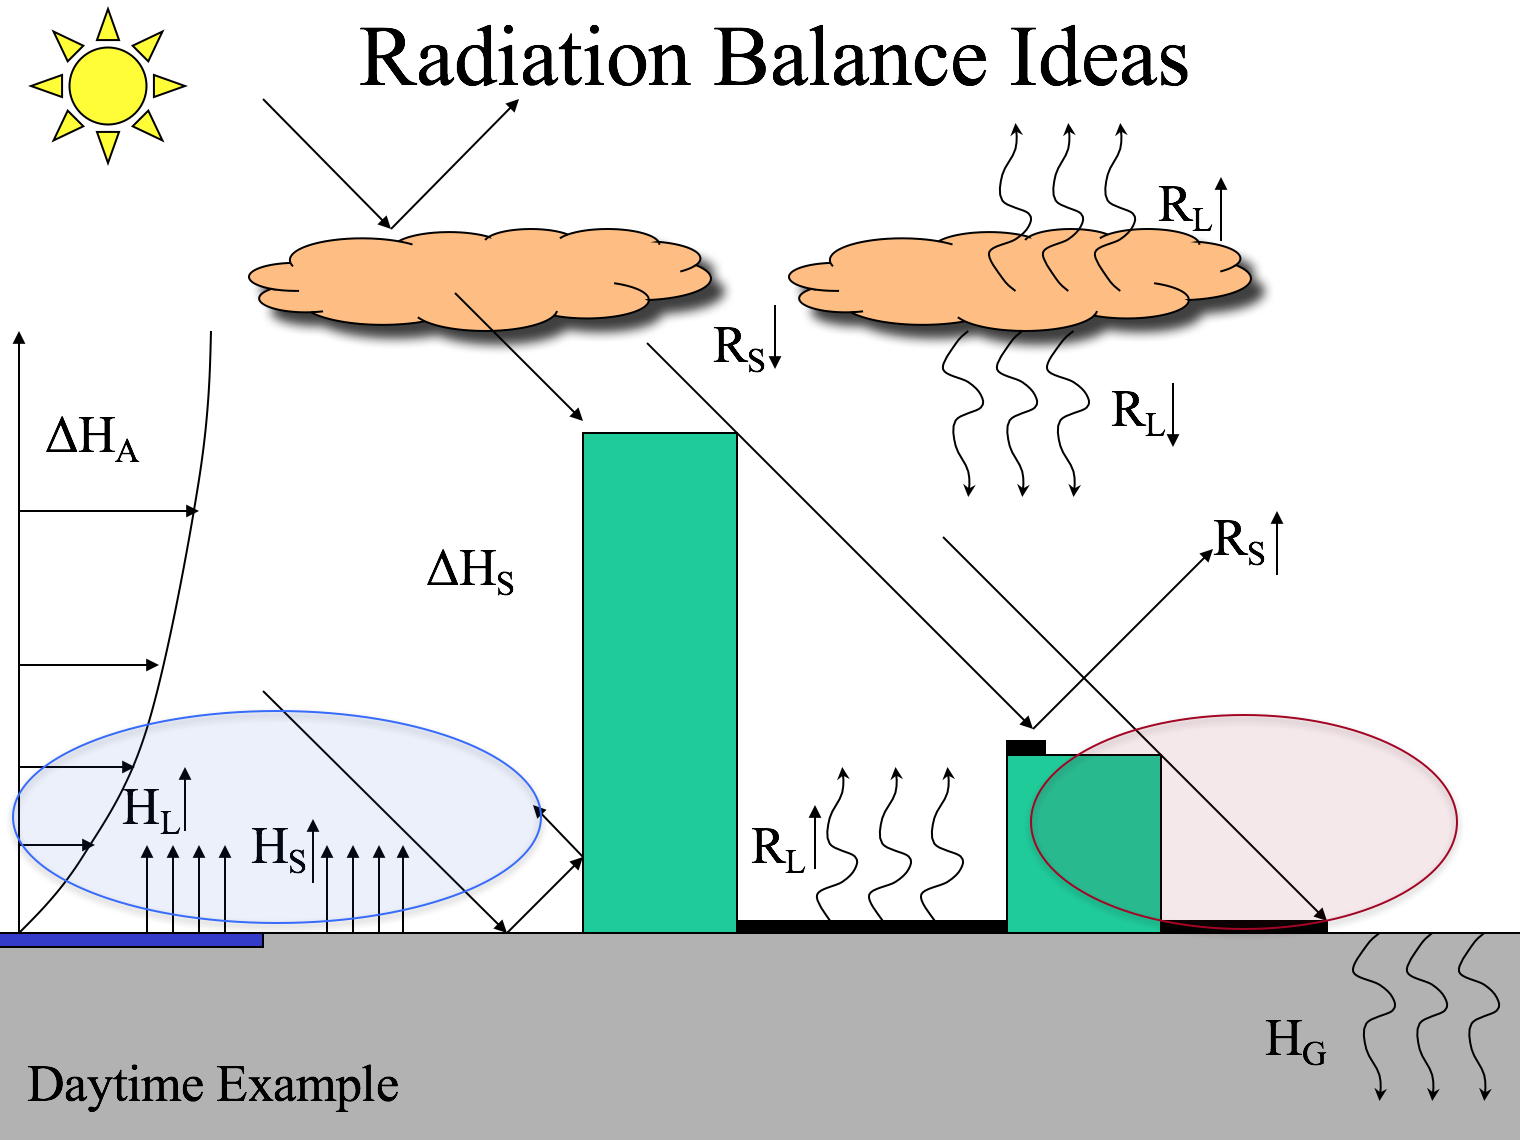
\includegraphics[width=1\textwidth]{rad1.png}
\end{figure}
\end{frame}

%------------------------------------------------
\begin{frame}{Near-Surface Energy Balance (SEB)}
Energy Balance at Earth's surface
\begin{itemize}
	\item Net radiation $\sim$ response fluxes
	\item Net radiation is composed of: incoming and outgoing solar and long-wave radiation
	\item Responsive fluxes include: sensible, latent, ground heat fluxes
\end{itemize}
\begin{figure}
	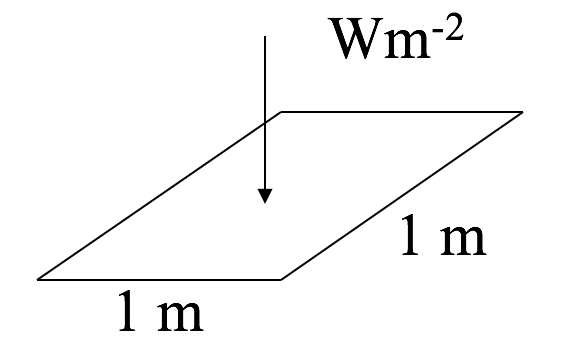
\includegraphics[width=0.4\textwidth]{rad2.png}
\end{figure}
\end{frame}

%------------------------------------------------
\begin{frame}{Near-Surface Energy Balance (SEB)}
Why is it important?
\begin{itemize}
	\item Energy/Water use (solar, geothermal)
	\item urban heat island
	\item Agriculture – freezing/thawing
	\item Air quality
	\item Thermodynamic/fluid mechanic interplay
\end{itemize}
\end{frame}

%------------------------------------------------
\begin{frame}{Radiation Balance - Ideal Surface}
One-dimensional balance sign convention
\begin{itemize}
	\item All radiative fluxes that point toward the surface are positive
	\item All non-radiative fluxes that point away from the surface are positive
	$$R_N = H_S + H_L + H_G$$
	\item We assume the surface is thin (no mass, textit{i.e.} heat capacity), flat, and horizontally homogeneous
\end{itemize}
\begin{figure}
	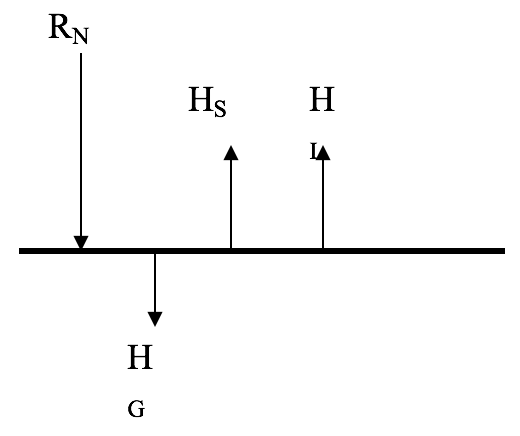
\includegraphics[width=0.48\textwidth]{rad3.png}
	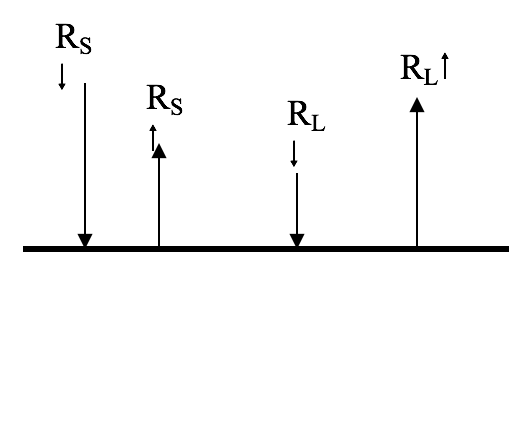
\includegraphics[width=0.48\textwidth]{rad4.png}
\end{figure}
\end{frame}

%------------------------------------------------
\begin{frame}{Radiation Balance - Ideal Surface}
All radiative fluxes that point toward the surface are positive
$$R_N = R_S \downarrow + R_S \uparrow + R_L \downarrow + R_L \uparrow$$
\begin{itemize}
	\item $R_s$ – shortwave radiation: $\sim 0.15-4.0\ \micro\metre$ (solar)
	\item $R_L$ – Longwave Radiation: $\sim 3.0-100\ \micro\metre$ (terrestrial)

\end{itemize}
\begin{figure}
	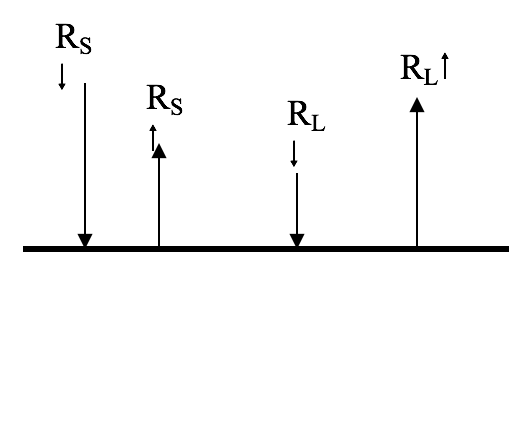
\includegraphics[width=0.35\textwidth]{rad4.png}
	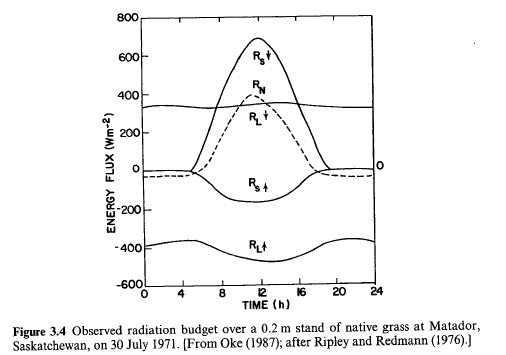
\includegraphics[width=0.63\textwidth]{rad5.png}
\end{figure}
\end{frame}

%------------------------------------------------
\begin{frame}{Surface Energy Budget}
\begin{figure}
	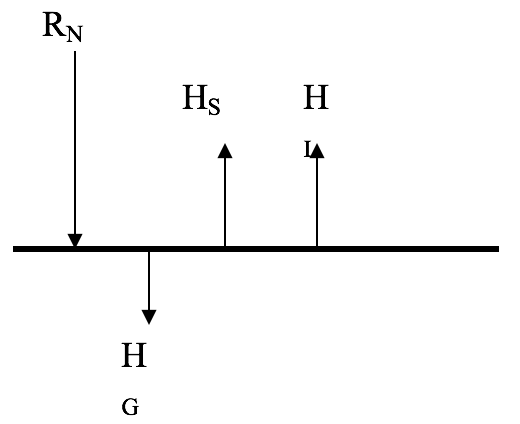
\includegraphics[width=0.49\textwidth]{rad6.png}
	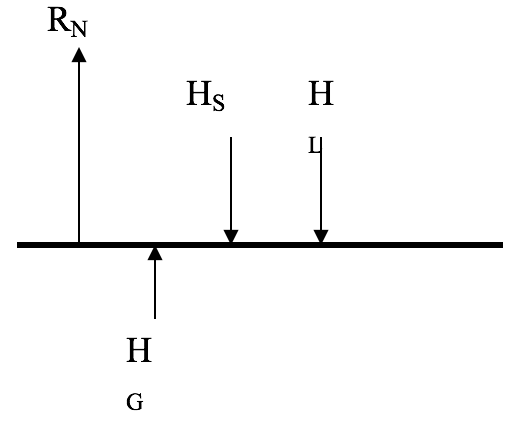
\includegraphics[width=0.49\textwidth]{rad7.png}
\end{figure}
Day (left) and Night (right) surface energy budget over land
\end{frame}

%------------------------------------------------
\begin{frame}{Surface Energy Budget}
$$\underbrace{R_N}_{\text{Forcing Term}} = \underbrace{H_S + H_L + H_G}_{\text{Response Terms}}$$
Types of energy fluxes at the surface
\begin{itemize}
	\item Net radiation ($R_N$)
	\item Sensible heat flux ($H_S$)
	\item Latent heat flux ($H_L$)
	\item Ground heat flux ($H_G$)
\end{itemize}
We assume the surface is thin (no mass, textit{i.e.} heat capacity), flat, horizontally homogeneous, and opaque.
\end{frame}

%------------------------------------------------
\begin{frame}{Surface Energy Budget - Finite Thickness Layer}
$$\underbrace{R_N}_{\text{Forcing Term}} = \underbrace{H_S + H_L + H_G + \Delta H_S}_{\text{Response Terms}}$$
\begin{itemize}
	\item We've now added heat storage: $\Delta H_S = \int \frac{\partial}{\partial t} (\rho CT) dz$
\end{itemize}
\begin{figure}
	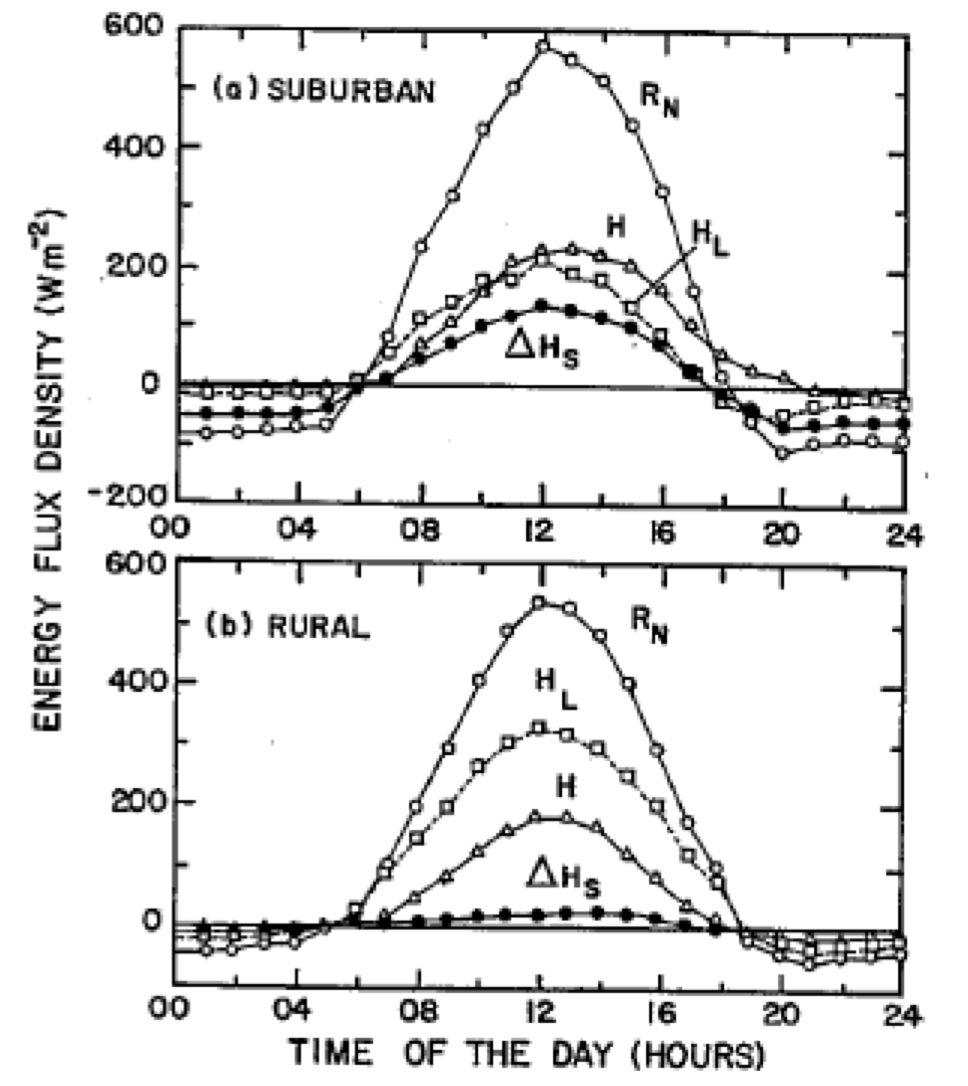
\includegraphics[width=0.43\textwidth]{rad8.png}
\end{figure}
\end{frame}

%------------------------------------------------
\begin{frame}{Surface Energy Budget - Finite Thickness Layer}
Storage can become particularly important in complex canopies such as urban areas and forests
\begin{figure}
	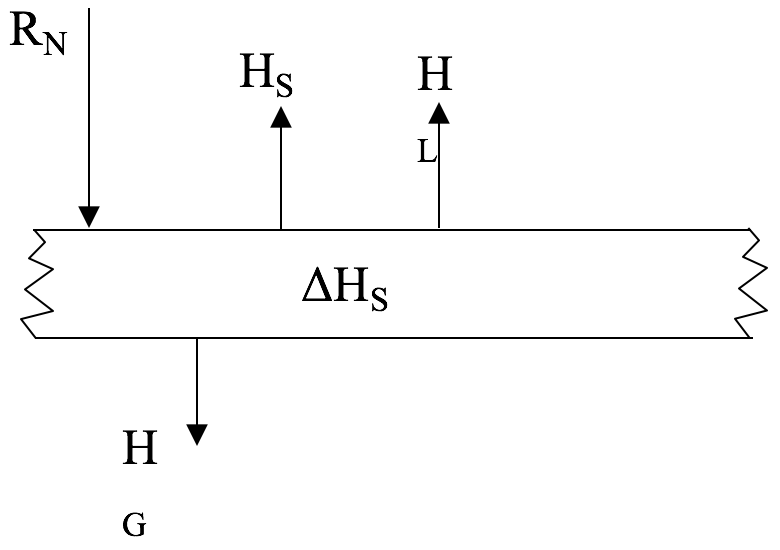
\includegraphics[width=0.45\textwidth]{rad9.png}\\
	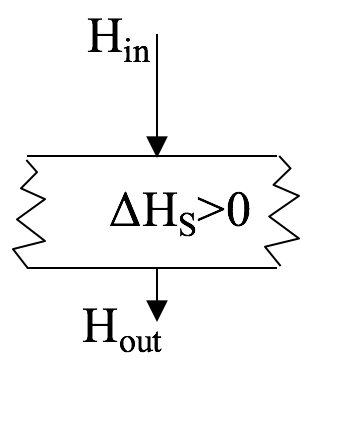
\includegraphics[width=0.25\textwidth]{rad10.png}
	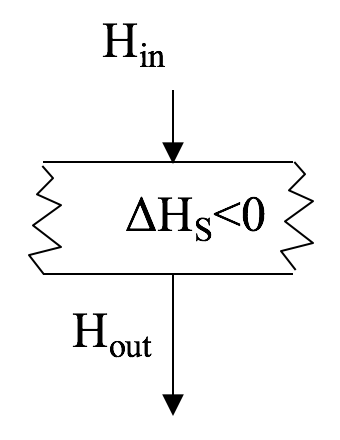
\includegraphics[width=0.25\textwidth]{rad11.png}\\
	\vspace{-10pt}
	\centering {\tiny Flux convergence (left) and flux divergence (right)}
\end{figure}
\end{frame}

%------------------------------------------------
\begin{frame}{Surface Energy Budget}
Surface energy budget in mountainous terrain - Switzerland
\begin{figure}
	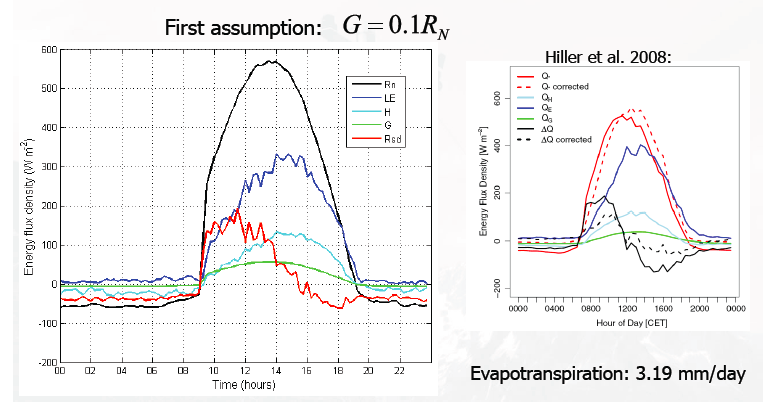
\includegraphics[width=1\textwidth]{rad12.png}\\
\end{figure}
\end{frame}

%------------------------------------------------
\begin{frame}{Urban Energy Balance}
\begin{figure}
	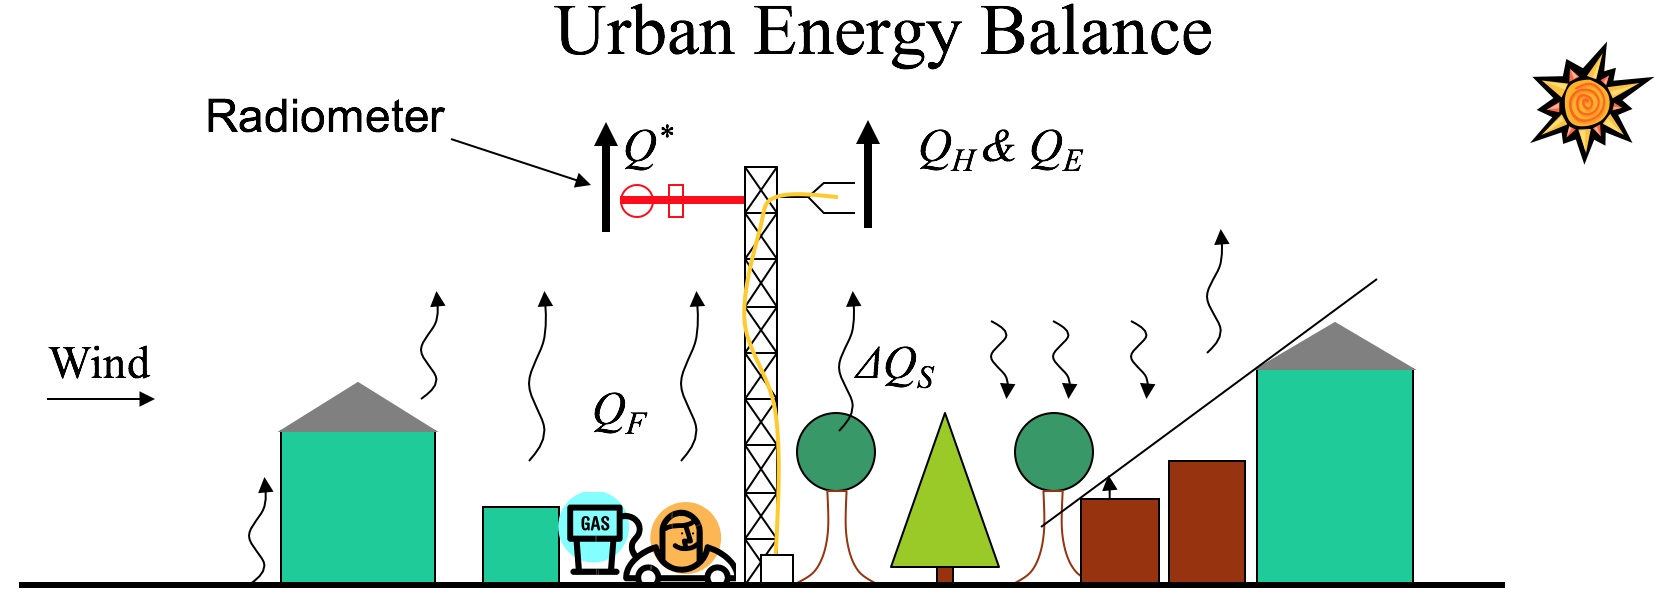
\includegraphics[width=1\textwidth]{rad13.png}\\
\end{figure}
$$Q^* = Q_F = Q_H + Q_E + \Delta Q_S$$
\begin{itemize}
	\item $Q^*$ = net all-wave radiation 
	\item $Q_F$ = anthropogenic heat flux
	\item $Q_H$ = latent heat flux
	\item $Q_E$ = sensible heat flux
	\item $\Delta Q_S$ = heat stored
\end{itemize}
\end{frame}

%------------------------------------------------
\begin{frame}{Urban Air Pollutant Transport}
\begin{figure}
	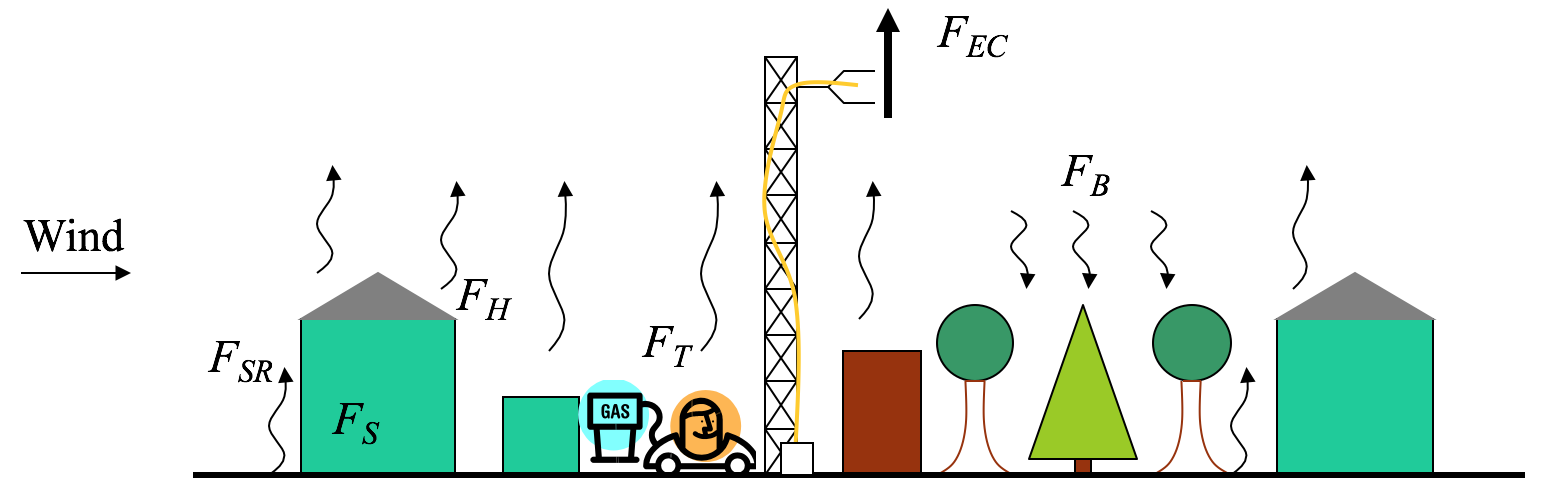
\includegraphics[width=1\textwidth]{rad14.png}\\
\end{figure}
$$F_{EC} = F_{SR} + F_B + F_T + F_H + F_S$$
\begin{itemize}
	\item $F_{SR}$ = flux of CO$_2$ due to soil respiration  
	\item $F_{B}$ = flux of CO$_2$ due to biogenic srcs (\textit{e.g.} photosynthesis)
	\item $F_T$ = flux of CO$_2$ due to traffic
	\item $F_H$ = flux of CO$_2$ due to heating
	\item $F_S$ = flux of CO$_2$ due to other household services
\end{itemize}
\end{frame}

%------------------------------------------------
\begin{frame}{Bowen Ratio}
$$\mathrm{BR} = \frac{\text{sensible}}{\text{latent}} = \frac{H_S}{H_L}$$
Estimate BR from balloon profile or local gradients
$$\mathrm{BR} \approx \gamma \frac{\partial \theta / \partial z}{\partial q_v / \partial z}$$
where the psychrometric $\gamma$ is given by
$$\gamma = \frac{C_p}{L_e} = 0.0004 (\gram_{\text{water}}/\gram_{\text{air}}) \kelvin^{-1}$$
\end{frame}

%------------------------------------------------
\begin{frame}{Bowen Ratio}
\begin{center}
Typical BR values\\
\begin{tabular}{ c c }
\hline
 Sea & 0.1 \\ 
 Irrigated crops & 0.2 \\  
 Grassland & 0.5  \\
 Semi-arid regions & 5\\
 Deserts & 10
\end{tabular}
\end{center}
\end{frame}

%------------------------------------------------

\end{document}

